\chapter{Symmetry-Maximizing Fair Values}

\section{Introduction}
The \textit{central limit order book (CLOB)} is one of the most common mechanisms for pairing orders between buyers and sellers in electronic marketplaces, and is used by most of the worlds biggest financial exchanges (NYSE, NASDAQ, LSE).
At any point of time, the CLOB keeps track of a list of prices and quantities that market
participants are willing to buy (bid) or sell (ask/offer) at. If there are any bids and asks that are overlapping, they are matched according to some matching rule and removed from the order book. What remains is a collection of bids and asks separated 
by some distance called the \textit{spread}. The CLOB changes over time as orders are matched, added, modified, or canceled, and its dynamics provide rich source of information about market sentiment.


Many attempts have been at modeling the dynamics of the CLOB, from the classical theory of point processes and SDEs to more modern treatments involving deep-learning and agent-based approaches.
The paper \cite{jain2024limitorderbooksimulations} provides a recent survey.

The goal of this project is to propose a new notion for the fair value of an exchange-tradeable asset given only the current state of the CLOB.


The bid side of the order book is typically encoded as list of prices $\{b_i\}$ at 
which orders are placed, where $b_0 > b_1 > ...$, and a list of total quantities 
$\{\beta_i\}$ at each price level. Likewise, the ask side has lists $\{a_i\}, \{\alpha_i\}$ 
for $a_0 < a_1 < ...$. The highest buy offer $b_0$ and lowest sell offer $a_0$ are called
 the \textit{best bid} (BB) and \textit{best ask/offer} (BO) respectively,
  and together they are called the BBO. The distance $s := a_0 - b_0$ is called the \textit{spread}, 
  and, since orders with crossing prices are matched and removed from the order book, it is strictly positive

\begin{figure}[h!]
    \centering
    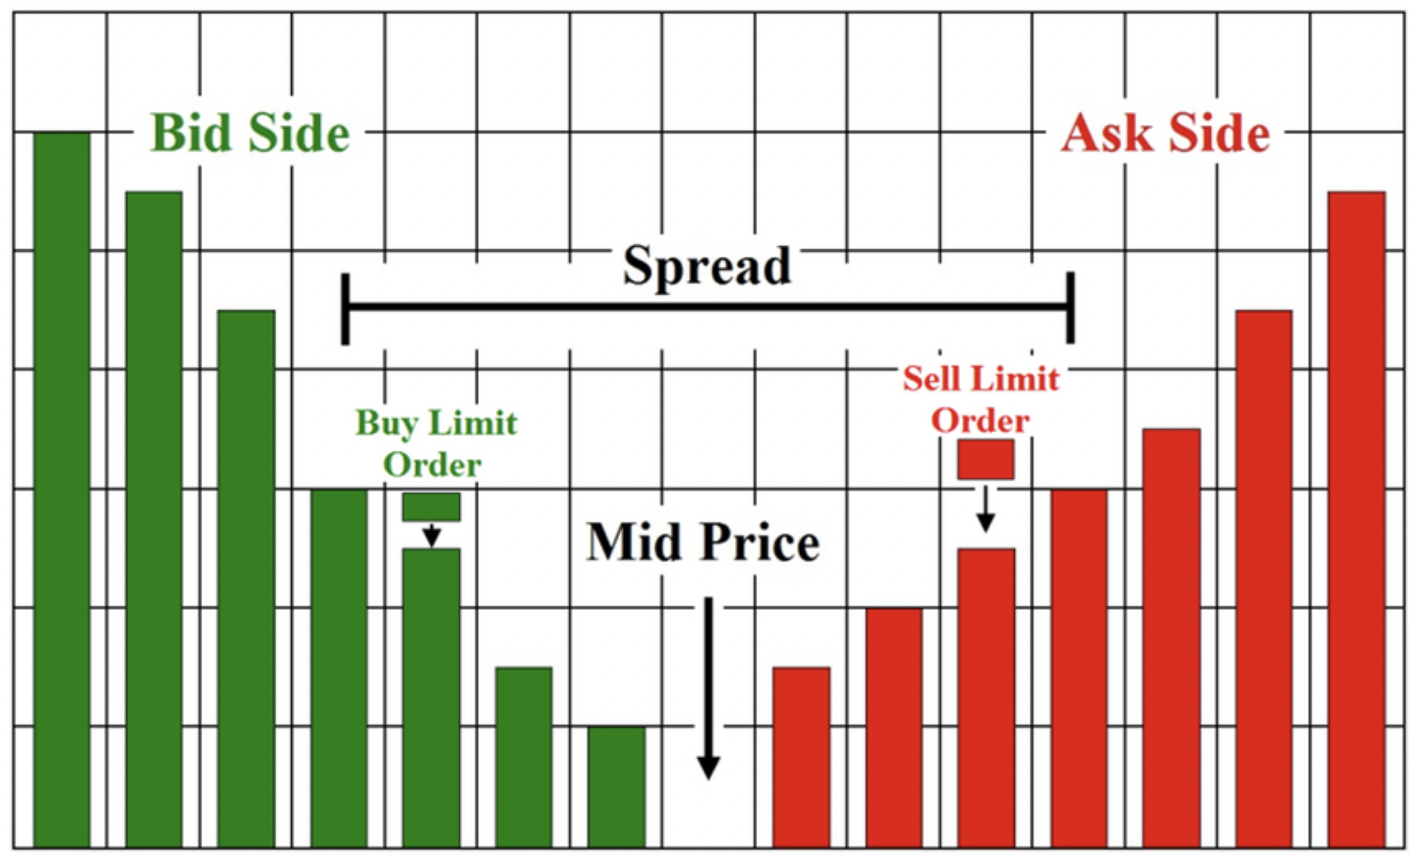
\includegraphics[width=0.7\textwidth]{images/ob_figure.png}
    \caption{Limit order book.}
    \label{fig:enter-label}
\end{figure}


Note in this view of the market, there is no one agreed upon price of the 
asset that people are willing to trade at. Instead, there is a range of prices
and quantities people are willing to buy at, and a range they are willing to
 sell at. Nonetheless, these bids and offers still provide some 
 information about what market participants think the asset is reasonably worth,
  the asset's \textit{fair value}: no reasonable person would place a bid higher
   than their fair value, nor an ask lower.

The goal of order book analysis is to infer what 
\textit{others believe the fair value is}, rather than attempting 
to compute it ourselves. Since most market activity is dominated by 
large market participants with significant informational, 
technological, and experiential advantages, this can sometimes be more
 reasonable than attempting to directly calculate a fair value ourselves.
  Of course, any estimate of the fair value from this order book analysis 
  can be aggregated with estimates from other sources if one desires.


A typical naive model for the fair value is just the \textit{mid price} 
$v_{m} = (b_0 + a_0) / 2$, the average of the best bid and best offer. But this does not
 incorporate any information about the sizes of the given price levels. 
 A more nuanced measure is the \textit{weighted mid price}:
%
\[v_w = \frac{b_0 \cdot \alpha_0 + a_0 \cdot \beta_0}{\beta_0 + \alpha_0} = v_m + s \cdot \frac{\beta_0 - \alpha_0}{\beta_0 + \alpha_0},\] 
%
which incorporates information about the imbalance in quantities available at the
 BBO. Namely, when there are many more bids than asks we might expect this 
 buying pressure to force the value of the asset upwards, and adjust our 
 fair value accordingly. 

The main downside of these two fair value estimates is that they only utilize 
information from the first price level. Some other heuristics like the 
\textit{volume-weighted average price} or the \textit{market-impact model} 
incorporate further price levels, but they often lack a rigorous motivation.
The volume-weighted average price averages prices across several levels using
the displayed quantities as weights, while a market-impact model estimates the
average execution price of a hypothetical market order that walks through the
book. 
For example, one might use
%
\[
    v_{\mathrm{VWAP}}(k)
    :=
    \frac{1}{2}
    \left(
        \frac{\sum_{i=0}^k b_i \beta_i}{\sum_{i=0}^k \beta_i}
        +
        \frac{\sum_{i=0}^k a_i \alpha_i}{\sum_{i=0}^k \alpha_i}
    \right),
\]
%
or, for a trade size $Q$, define $I_b(Q)$ and $I_a(Q)$ to be the average
execution prices of selling or buying $Q$ units against the book, and set
%
\[
    v_{\mathrm{impact}}(Q) := \frac{I_b(Q) + I_a(Q)}{2}.
\]

We aim to develop a metric of the fair value that captures more nuanced 
information about the \textit{shape} of the order book that is optimal in some probabilistic 
sense, and which reduces to the above heuristics under natural assumptions.
 In this way, we provide a rigorous mathematical foundation for the aforementioned 
 heuristics while also developing a large new class of potential fair value metrics. 

Our idea was to first view the bid side of the order book and the ask side of 
the order book as two separate distributions $\mu_b, \mu_a$. One way of doing 
this is to view each quantity (or order) as a unit mass on the order book 
(and then possibly normalize):
%
\begin{equation}
    \mu_b \propto \sum_{i} \beta_i \cdot \delta_{b_i}, \qquad \mu_a \propto \sum_{j} \alpha_j \cdot \delta_{a_j}.
    %
    \label{eqn:mua_mub_proportional}
\end{equation}
%
\noindent Instead of treating each quantity identically, we could also choose to weight
 the orders according to some scheme. Since it seems likely that orders near the spread 
 are more informed, it is natural to weight these orders more. Namely, by introducing a 
 discount $\lambda \in (0,1]$, we could choose to add more mass to the larger bids and 
 the smaller asks, the orders nearer to the spread:
%
\begin{equation}
    \mu_b \propto \sum_{i} \lambda^{-b_i} \cdot \beta_i \cdot \delta_{b_i}, \qquad \mu_a \propto \sum_{j} \lambda^{a_j} \cdot \alpha_j \cdot \delta_{a_j}.
    \label{eqn:mua_mub}
\end{equation}
%
In the rest of this note, we will not assume $\mu_a, \mu_b$ take any
 particular form, but these two examples are good to have in mind.

To try to generalize our heuristics, consider the simple situation where the bid
and asks books are perfect mirror images of each other, separated possibly by some spread. In this case, buying and selling pressures are exactly equal, so the mid price $v_m$ is a natural candidate for the fair value. In particular, it is the point around which the two distributions are mirror images: reflecting the ask book across the mid price gives exactly the bid book. In other words, $v_m$ solves:
%
\begin{equation}
    v_s = \argmin_{c \in \R} \; d(\mu_a(\cdot + c), \; \mu_b(c - \cdot)),
    \label{eqn:optimization_problem}
\end{equation}

%
\noindent for any metric $d$ on a suitable space of probability distributions.
 In general, we will not have such nice symmetry, but we can still seek to 
 solve \eqref{eqn:optimization_problem} for a fixed metric $d$. 
 We will call the solution $v_s$ the \textit{symmetry-maximizing value}, and 
 it implictly depends on $d$. A visualization of this procedure is given in Figure~\ref{fig:sym-fv-viz}.

 % fair value viz
\begin{figure}[h!]
    \centering
    \begin{subfigure}[t]{0.48\textwidth}
        \centering
        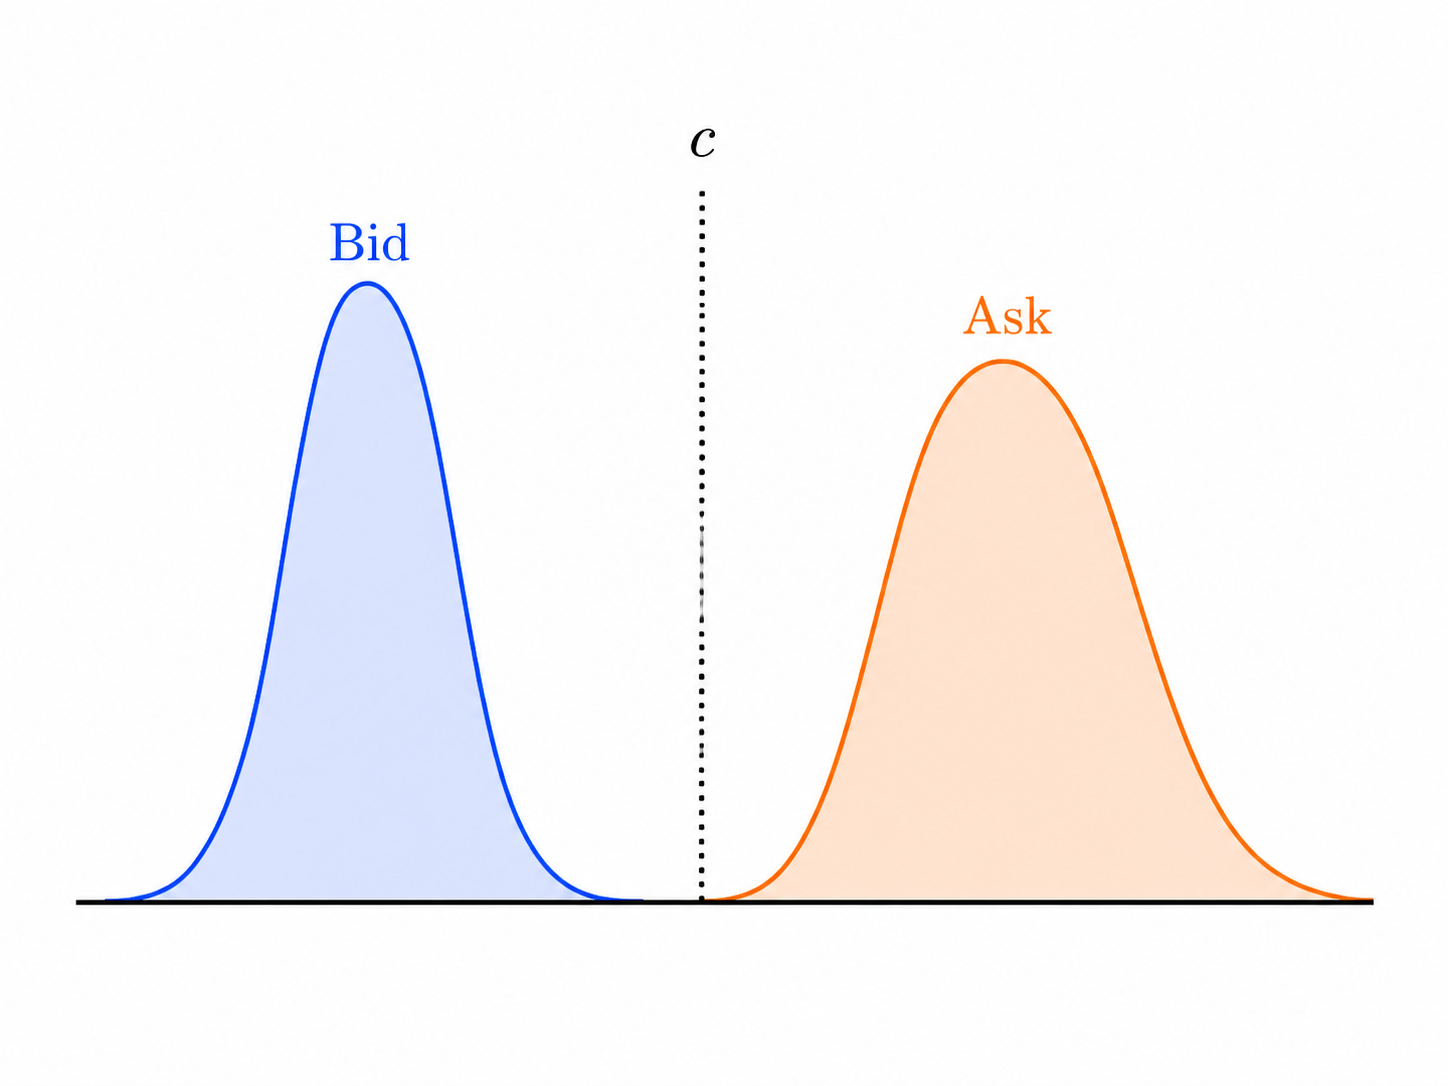
\includegraphics[width=\linewidth, height=0.31\textheight, keepaspectratio]{images/sym_fv_viz1.png}
        \caption{Original order book.}
        \label{fig:sym-fv-viz-1}
    \end{subfigure}
    \hfill
    \begin{subfigure}[t]{0.48\textwidth}
        \centering
        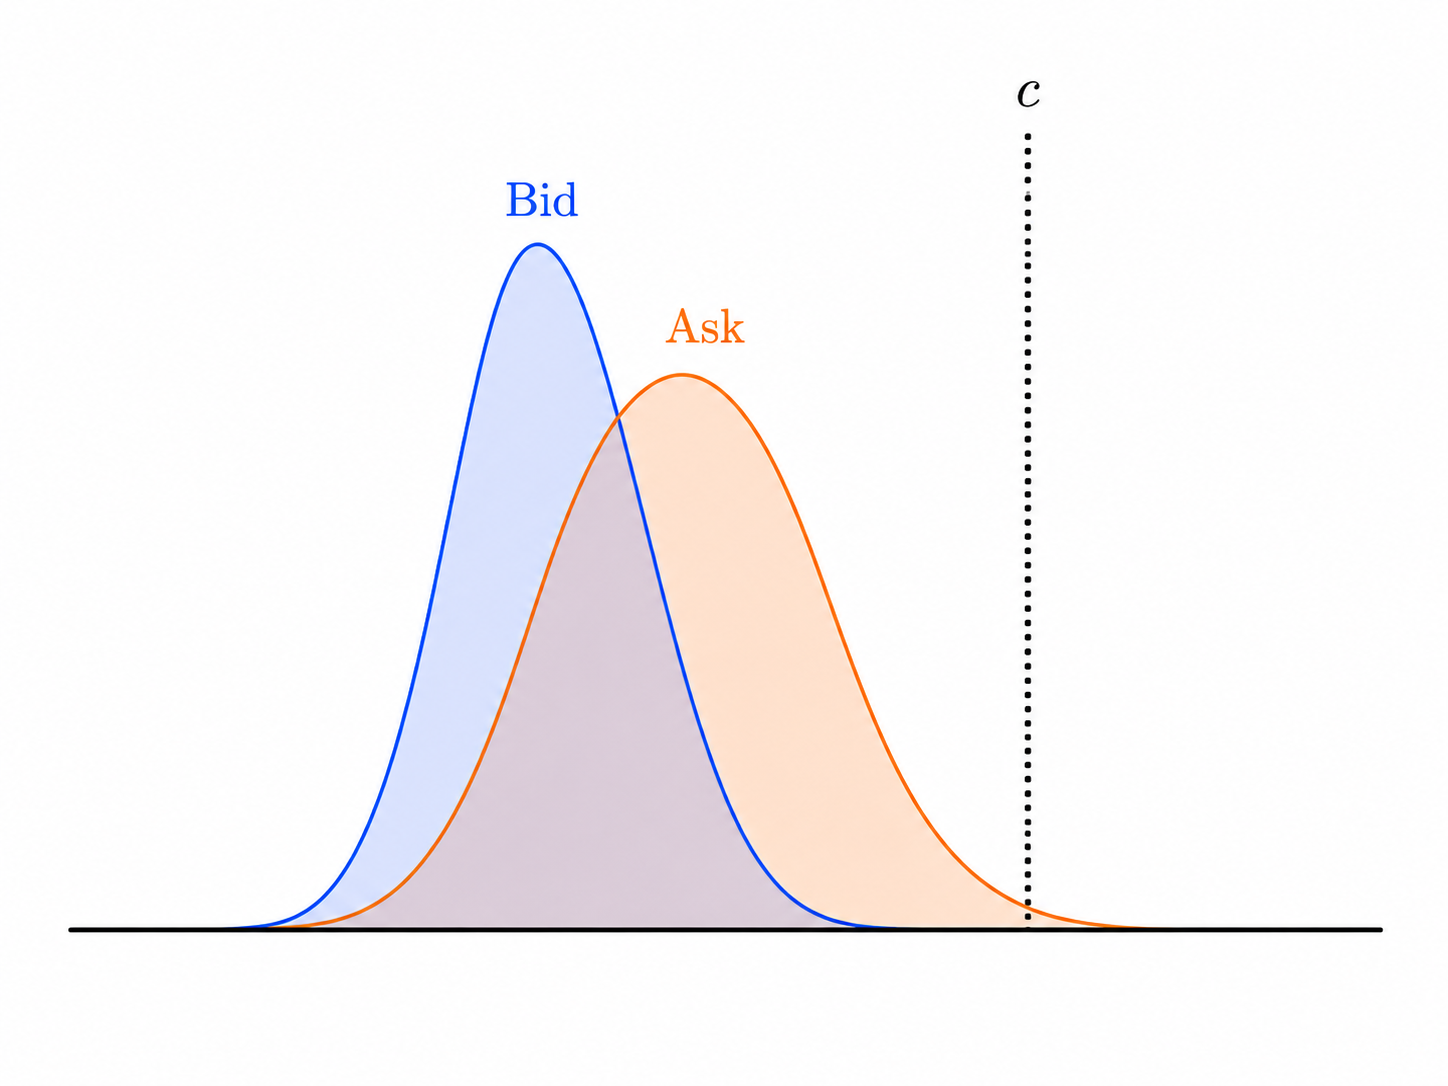
\includegraphics[width=\linewidth, height=0.31\textheight, keepaspectratio]{images/sym_fv_viz2.png}
        \caption{Reflected ask book across $c$.}
        \label{fig:sym-fv-viz-2}
    \end{subfigure}
    \caption{Visualization of the symmetry-maximizing fair value. The ask
    book is reflected across the candidate fair value $c$, and the distance between the
    reflected ask book and the bid book is measured by some metric $d$.}
    \label{fig:sym-fv-viz}
\end{figure}
%end fig




%%%%%%%%%%%%%%%%%%%%%%%%%%%%%%%%%%%%%%%%%%%%%%%%%%%%
% Modeling A Single Order Book 
%%%%%%%%%%%%%%%%%%%%%%%%%%%%%%%%%%%%%%%%%%%%%%%%%%%%
\newpage
\section{A Simple Model For Market Makers}

The following model is overly simplistic, and is not intended as a literal description of order-book
formation. Rather, it is a stylized mechanism showing how a symmetry-based fair
value arises when the two sides of the book are generated by agents placing bid
and ask quotes around latent fair values. In this model, estimating the fair
value becomes a problem of pairing bids and asks in a natural way, and then
approximating the latent fair-value distribution by its empirical distribution.

Market makers supply liquidity by placing buy and sell orders around their
own estimates of an asset's fair value. If a market maker has no directional
preference and current buying and selling pressures are balanced, it is natural
to model their quotes as being placed symmetrically around some latent fair value
$v$. Thus, a simple paired-order model takes bids and asks of the form
%
\[bid = v - h, \qquad ask = v + h,\]
%
where $h$ is a latent half-spread specific to that quote pair, reflecting the
agent's uncertainty, inventory concerns, or required compensation for supplying
liquidity. More generally, if buying and selling pressures are not balanced, we
may expect market makers to shift their bids and asks asymmetrically around their
fair values.
%
\[bid = v - \theta^{-1}h, \qquad ask = v + (1-\theta)^{-1}h,\]
%
where $\theta \in (0,1)$ is an exogenous imbalance parameter. Namely, as
$\theta$ approaches zero, selling pressure is interpreted as increasing, and
market makers move their bids farther away from the fair value to protect
against adverse selection during future price movements. When $\theta$
approaches one, the analogous effect occurs on the ask side.
Formally, we study the following generative model:
%
\begin{align*}
    v &\sim \mu \in \mathbb{P}(\mathbb{R})  && \text{(fair value distribution)} \\
    h &\sim \nu \in \mathbb{P}((0,\infty)) && \text{(half-spread distribution)} \\
    %\epsilon_i, \eta_i &\in N(0, \sigma^2) && \text{(noise)} \\
    \theta &\in (0,1) && \text{(imbalance)}.
\end{align*}
%
\[ \text{bid} = v - \theta^{-1} h, \qquad \text{ask} = v + (1-\theta)^{-1} h. \]


\noindent Note that the above implies:
%
\[v = \theta \cdot \text{bid} + (1-\theta) \cdot \text{ask}, \qquad h = \theta(1-\theta) \cdot (\ask - \bid).\]
%
 Thus, if we knew which bid was paired with each ask, we could aggregate 
 these to get reasonable estimates of the fair value and half-spread 
 distributions:

 %
\[\hat{\mu} := \frac{1}{n} \sum_{i=1}^n \delta_{\theta \cdot \bid_i + (1-\theta) \cdot \ask_i}, \qquad \hat{\nu} = \frac{1}{n} \sum_{i=1}^n \delta_{\theta(1-\theta)(\ask_i - \bid_i)}.\]
 %
 \noindent We start by getting some simple bounds on the basic moments of 
 these distributions:

 \begin{lemma}
 Suppose that $\bid_n \leq ... \leq \bid_1 \leq \ask_1 \leq ... \leq \ask_n$. Then if we define $\mu_a, \mu_b$
as in \ref{eqn:mua_mub_proportional}, regardless of how bids and asks are paired up, we have:
\[m_2(\hat{\mu}) = \theta \cdot m_2(\mu_b) + (1-\theta) \cdot m_2(\mu_a), \qquad m_2(\hat{\nu}^\tau) = \theta (1-\theta)(m_2(\mu_a) - m_2(\mu_b)).\]
%
\noindent where $m_2(\mu)$ is the standard mean. Moreover, if for a permutation $\tau$ of $[n]$ we let:
%
\[\Cov_\tau(\bid, \ask) := \frac{1}{n} \sum_{i=1}^n [\bid_i - m_2(\mu_b)]\cdot[ \ask_{\tau(i)} - m_2(\mu_a)],\]
%
\noindent be the empirical covariance between the bid and ask prices under pairing $\tau$, then:
%
\begin{equation*}
    \Cov_{\mathrm{id}}(\bid, \ask) \leq  \frac{1}{2\theta(1-\theta)}
    \Big[\Var(\hat{\mu}_\tau) - \left(\Var(\theta \mu_b) + \Var((1-\theta)\mu_a)\right) \Big] 
    \leq \Cov_{\rho}(\bid, \ask).
\end{equation*}
%
\begin{equation*}
    \Cov_{\mathrm{id}}(\bid, \ask) 
    \leq  -\frac{1}{2}\Big[\frac{\Var(\hat{\nu}_\tau)}{\theta^2(1-\theta)^2}
    - \left(\Var( \mu_b) + \Var(\mu_a)\right) \Big] 
    \leq \Cov_{\rho}(\bid, \ask).
\end{equation*}
%
\noindent where $\rho(i) = n+1 - i$ is the reverse permutation, and $\hat{\mu}_\tau, \hat{\nu}_\tau$ are 
the empirical distributions under the pairing $(\bid_i, \ask_{\tau(i)})_{i=1}^n$. Namely, the minimizer/maximizer are the ``inside-out" and ``left-to-right" pairings of
 bids, asks respectively.

\label{lem:estimated_fv_and_spread_mean_and_variance}
 \end{lemma}
 

\noindent Likewise, if we knew the pairings of bids and asks and were
 interested in the $p^{th}$ mean $m_p(\mu) := \argmin_c \E_\mu (X-c)^p$ we 
 could approximate it by:
 %
\[m_p(\hat{\mu}) = \argmin_c \sum_{i=1}^n | c - \theta \cdot \text{bid}_i - (1-\theta) \cdot \text{ask}_i|^p. \]
 %
 \noindent As we will see later, this has the same form as our symmetric fair-value objective \eqref{eqn:wp_imbalanced_symmetric_fair_value} once a pairing of bids and asks has been chosen. 
 Since the identity of the issuer of each order is unknown, the main problem becomes choosing a reasonable pairing. 
 Equivalently, the symmetry-maximizing value can be viewed as a relaxation of this latent pairing problem.

 Of course, a real order book need not admit a literal one-to-one
decomposition into bid/ask pairs. The paired model should instead be viewed as
a finite approximation to a coupling between the bid-side and ask-side
distributions.

%%%%%%%%%%%%%%%%%%%%%%%%%%%%%%
% Determining optimal pairing of bids and asks %
%%%%%%%%%%%%%%%%%%%%%%%%%%%%%%%%%
\subsection{Determining optimal bid/ask pairing}

Suppose we have $n$ bids $\bid_1 \geq ... \geq \bid_n$ and $n$ asks $\ask_1 \leq ... \leq \ask_n$. Pairing these up amounts to choosing a permutation $\tau \in S_n$ and pairing $\bid_i$ with $\ask_{\tau(i)}$. If we assume this is the true pairing, the above generative model specifies exactly its probability distribution. Finding the optimal way of pairing up asks and bids then amounts to solving:
%
\begin{align*}
    & \argmax_{\tau \in S_n} \P_{v,h}\left((\bid_i, \ask_{\tau(i)})_{i=1}^n\right) \\
    %
    & = \argmax_{\tau \in S_n} \sum_{i=1}^n \log\left(\P_{v,h}(\bid_i, \ask_{\tau(i)})\right) \\
    %
    & = \argmax_{\tau \in S_n} \sum_{i=1}^n \log\left(\P_h(\theta (1-\theta) \cdot (\ask_{\tau(i)} - \bid_i)\right) + \log\left( \P_v(\theta \bid_i + (1-\theta) \cdot \ask_{\tau(i)})\right).
\end{align*}
%
\noindent If we assume we have densities $\P_h = e^{f(x)} \; dx$ and 
$\P_v = e^{g(x)} \; dx$ then this reduces to:
%
\[= \argmax_{\tau \in S_n} \sum_{i=1}^n f\Big(\theta(1-\theta) \cdot (\ask_{\tau(i)} - \bid_i) \Big ) + g\Big(\theta \cdot \bid_i + (1-\theta) \cdot \ask_{\tau(i)}\Big). \]
%
\noindent The next lemma gives conditions under which this score is maximized
when bids and asks are paired in the natural way: from inside the spread
outwards. Towards this end, we introduce the discrete differences
%
\[\Delta_r f(z) := f(z + r) - f(z).\]
%
\noindent A function $f$ is concave if and only if for any $r > 0$ then
 $\Delta_r f$ is nonincreasing. Thus in the case of concave functions,
  the second discrete derivative $\Delta_t \Delta_r f$ is nonpositive, 
  and its magnitude in a sense quantifies the level of concavity. The 
  following identifies the optimal pairing in the case $\mu$ is 
  sufficiently ``more log-concave" than $\nu$ or vice versa.

\begin{lemma}
    Suppose $\mu = N(0, \sigma^2)$ and $\nu = e^{f(x)}$. If for all $z \in \R$ 
    and $t,r > 0$:
    %
    \begin{equation}
         \Delta_t \Delta_r f(z) \geq - \frac{1}{\theta(1-\theta)\sigma^2} \cdot rt.
         \label{eqn:gaussian_concavity_condition}
    \end{equation}

    %
    \noindent If $\bid_n \leq ... \leq \bid_1 \leq \ask_1 \leq ... \leq \ask_n$ then:
        %
    \[\mathrm{id} = \argmax_{\tau \in S_n} \sum_{i=1}^n f\Big(\theta(1-\theta) \cdot (\ask_{\tau(i)} - \bid_i) \Big ) + g\Big(\theta \cdot \bid_i + (1-\theta) \cdot \ask_{\tau(i)}\Big). \]
    %
    \noindent Namely, the optimal pairing is moving from inside the spread outwards.
     Moreover, if the reverse inequality is true the optimal pairing is from left to 
     right.

    \label{lem:optimal_pairing_bids_and_asks_gaussian}
\end{lemma}

\noindent Note, the right hand side of equation \eqref{eqn:gaussian_concavity_condition} is just the second 
discrete derivative of $g(x) = -\frac{x^2}{2\sigma^2}$, the log-density of the Gaussian. Thus, the 
condition is saying that our fair value distribution is more log-concave than our spread distribution in a strong way.

\begin{remark}
    If $f$ is twice differentiable, then a Taylor series expansion shows
     $\Delta_t \Delta_r f(z) \approx rt \cdot f''(z)$. Thus the 
     assumption of the theorem roughly says the second derivative is bounded 
     below by some sufficiently large constant.
\end{remark}

\begin{remark}
    In practice, since bids and asks can only be placed at discrete tick-sizes 
    we could effectively relax the assumptions to only $z,t,r \in \mathbb{Z}_{> 0}$.
\end{remark}

\begin{example}
    In particular, one natural choice is $\nu = \mathrm{Gamma}(\lambda, k)$. Here:
    %
    \[f(x) = -\lambda x + (k-1) \log(x) + C_{\lambda, k} \quad \to \quad \Delta_t\Delta_r f(x) = (k-1) \log\bigg(1 - \frac{rt}{(x+r)(x+t)}\bigg). \]
    %
    \noindent In the exponential case ($k=1$) or when $k < 1$ then assumption
     \eqref{eqn:gaussian_concavity_condition} is trivially satisfied because 
     the second discrete derivative is nonnegative. Otherwise, if $k > 1$ then $\Delta_t \Delta_r f(x) \to - \infty$ as $x \downarrow 0$,
     so the assumptions are not met. In this regime, the Gamma distribution has sufficient mass away from zero, so
     large spreads are not as heavily penalized, and the optimal pairing is no longer necessarily from inside out.
\end{example}

\noindent Note that our above proof of Lemma \ref{lem:optimal_pairing_bids_and_asks_gaussian} actually shows something slightly stronger.

\begin{corollary}
    If $\bid_n \leq ... \leq \bid_1 \leq \ask_1 \leq ... \leq \ask_n$ and for all $t,r > 0$:
    %
    \[\Delta_{\theta t} \, \Delta_{(1-\theta) r} \, f(z) \geq \Delta_{r} \Delta_{t} g(w),\]
    %
    \noindent for $z \in [0, \ask_n - \bid_n]$ and $w \in [\bid_n, \ask_n]$, then we can see:
    %
    \[\mathrm{id} = \argmax_{\tau \in S_n} \sum_{i=1}^n f\Big(\theta(1-\theta) \cdot (\ask_{\tau(i)} - \bid_i) \Big ) + g\Big(\theta \cdot \bid_i + (1-\theta) \cdot \ask_{\tau(i)}\Big). \]
    %
    \noindent Namely, the optimal pairing is moving from inside the spread outwards.
        \label{cor:optimal_pairing_bids_and_asks_general}
\end{corollary}


Above, we show that under this simple model of market-making, 
the optimal pairing of bids and asks are the two naive ones: either 
pairing from the ``inside-out" by pairing the best bid with the best offer, and so on, or pairing from 
``left to right", pairing the worst bid with the best offer. In Section \ref{sec:stability_fv} below, 
we will show such pairings naturally arise from our proposed symmetry-maximizing fair 
value under a canonical choice of distance metric: the $W_2$ Wasserstein metric. 


%%%%%%%%%%%%%%%%%%%%%%%%%%%%%%%%%%%%%%%%%%%%%%%%
 % Studying Order Book Shape 
%%%%%%%%%%%%%%%%%%%%%%%%%%%%%%%%%%%%%%%%%%%%%%%%
\section{Incorporating Order Book Shape}
\label{sec:incorporating_order_book_shape}


There are many natural measures of ``distance" between probability measures: total
variation, Jensen-Shannon divergence, and $\chi^2$-type distances. These are less
suitable for the present application because they compare mass at fixed locations, 
making them sensitive to small shifts in order prices or quantities. Since financial 
markets are inherently noisy, we want a metric that is more robust under such perturbations,
and which incorporates more of the \textit{geometry} of the order book than these pointwise
comparisons. 

The Wasserstien distance is the natural candidate. In this section, we aim to study
how the symmetry-maximizing fair value behaves when the underlying metric $d$ is chosen to be this distance. 
In Theorem~\ref{thm:wasserstein_solution}, we characterize the symmetry-maximizing fair value under the Wasserstein metric, 
and in Lemma~\ref{lem:fv_continuity} we quantify the stability of this fair-value with respect to small changes 
of the order book. 


% Wasserstein %%%%%%%%%%%%%%
\subsection{Wasserstein p-metric}

This metric comes from the theory of optimal transport. It measures how
 difficult it is to convert one distribution into another by transporting 
 it ``piece by piece". The goal is to find a transportation plan that 
 requires the least total distance the mass must be transported. 
 Formally, its defined as:
%
\[d_{W_p}(\mu, \nu) := \left( \inf_{(X,Y) \in \Pi(\mu, \nu)} \E |X-Y|^p \right)^{1/p},\]
%
\noindent where $\Pi(\mu, \nu)$ is the space of all couplings of $\mu, \nu$, joint distributions of $(X,Y)$ that have marginals $\mu, \nu$ respectively. Namely, for each $x \in \R$ our coupling $\pi(x, \cdot)$ specifies where in $\nu$ the mass $\mu(x)$ must be sent, and we search for a way of doing this that minimizes the total transportation distance. The below theorem shows \eqref{eqn:optimization_problem} takes the form of a simple convex optimization problem. First, we introduce some notation for equation \eqref{eqn:mua_mub}.
%
\begin{align*}
    b_i & := \frac{\sum_{j=1}^i\lambda^{b_j} \cdot \beta_j}{\sum_{j=1}^n \lambda^{b_j} \cdot \beta_j} \qquad a_i  := \frac{\sum_{j=1}^i\lambda^{a_j} \cdot \alpha_j}{\sum_{j=1}^m \lambda^{a_j} \cdot \alpha_j} \qquad  a_0 = b_0 = 0\\
    \\
    z_k & := \inf \{a_i : a_i > z_{k-1}\} \cup \{b_i : b_i > z_{k-1}\} \qquad \Delta z_\ell := z_\ell - z_{\ell - 1} \qquad  z_0 := 0.
\end{align*}
%

\noindent Namely, the $a_i, b_i$ keep track of our cumulative distribution functions of the bid and ask distributions as we move away from the best bid and best offer, and the $z_k$ are the order statistics of these combined values. Moreover, define $f(k) = i$ if $[a_{i-1}, a_i)$ is the unique interval of this kind containing $z_k$. Likewise define $g(k) = i$ if $z_k \in [b_{i-1}, b_i)$.
%
Now we are ready to relate these quantities to the symmetry-maximizing fair value. 
%
\begin{theorem}
    For any $p \geq 1$, $v_s$ solves the convex optimization problem: 

    \begin{equation}
    v_s = \argmin_{c > 0} \sum_{\ell = 1}^{m+n} \Delta z_\ell \cdot |2c - b_{f(\ell)} - a_{g(\ell)}|^p.
    \end{equation}

    \noindent Moreover, in the case $p = 2$ the explicit solution is:
    %
    \begin{equation}
        v_s = \frac{1}{2} \Big( m_2(\mu_a) + m_2(\mu_b)\Big).
        \label{eqn:explicit_soln_sym_fv}
    \end{equation}
    %
    \label{thm:wasserstein_solution}
\end{theorem}
%
\begin{remark}
    As discussed in Section \ref{sec:stability_fv} we see \eqref{eqn:explicit_soln_sym_fv} is just the mean of the $W_2$ barycenter of $\mu_a, \mu_b$. Thus we can take the barycenter as an estimate of the full fair-value distribution rather than just taking its mean as this point estimate.
\end{remark}

%%%%%%%%%%%%%%%%%%%%%%%%%%%%%%%%%%%%%%%%%%
% Introducing Imbalances 
%%%%%%%%%%%%%%%%%%%%%%%%%%%%%%%%%%%%%%%%%%
\section{Introducing Quantity Imbalances}
\label{sec:quantity_imbalances}

A natural criticism of our work in Section \ref{sec:incorporating_order_book_shape}
 is that we lose information about imbalance between the bid and ask
  sides of the order book, imbalances which fair value estimates 
  like the weighted mid $v_w$ discussed earlier seek to exploit. 
  Thus, it may only be a decent estimate of the fair value in 
  situations when the total number of bids and total number asks
   are roughly equal. In this section, we discuss a way of expanding 
   our previous approach to incorporate this kind of information. 

In this section, we drop our assumption that $\mu_a, \mu_b$ be 
probability measures, so they can take unnormalized forms like in
equation \eqref{eqn:mua_mub}. One simple measure of imbalance is 
then just the following ratio of the total masses $m_a, m_b$ of 
these measures:
%

\begin{equation}
    \theta = \frac{m_a}{m_a + m_b}.
    \label{eqn:imbalance_ratio_theta}
\end{equation}

%

\noindent In the case of the unnormalized measures 
\ref{eqn:mua_mub_proportional}, this is just the ratio of the total 
volume on the bid book and the total volume on the ask book. 
Using this, we can extend \ref{eqn:optimization_problem} in a way
 that incorporates the imbalances in the bid and ask books:
%
\begin{align}
        v^\theta_s & = \argmin_{c > 0} d\left(\frac{\mu_b[(c - \cdot) / 2\theta] }{m_b}, \; \frac{\mu_a[ (\cdot + c) / 2(1-\theta)]}{m_a}\right).
        %
        \label{eqn:imbalanced_optimization_problem}
\end{align}
%
\noindent We then have the corresponding extension of 
Theorem~\ref{thm:wasserstein_solution}, which in the case $p=2$ 
just says we replace the standard average in 
Theorem~\ref{thm:wasserstein_solution} by an average weighted
 by the imbalance.

\begin{theorem}
    Let $\theta \in (0,1)$. Then for any $p \geq 1$, $v^\theta_s$ solves the 
    convex problem: 
%
\begin{equation}
   v^\theta_s = \argmin_{c > 0} \sum_{\ell = 1}^{m+n} \Delta z_\ell \cdot |2c - 2\theta \cdot b_{f(\ell)} - 2(1-\theta) \cdot a_{g(\ell)}|^p.
   \label{eqn:wp_imbalanced_symmetric_fair_value}
\end{equation}
%
\noindent Moreover, in the case $p = 2$ the explicit solution is:
%
\begin{equation}
    v^\theta_s = \theta \cdot m_2(\mu_b) + (1-\theta) \cdot m_2(\mu_a).
    \label{eqn:w2_imbalanced_symmetric_fair_value}
\end{equation}
    \label{thm:imbalanced_wasserstein_solution}
\end{theorem}

%
\begin{remark}
    In the case there is only one price level and \eqref{eqn:mua_mub_proportional}, or 
    when $\mu_a, \mu_b$ only put mass on the first price level proportional to the quantity, 
    and we choose $\theta$ by \eqref{eqn:imbalance_ratio_theta} then $v_s^\theta = v_w$, 
    the weighted mid price.
\end{remark}


\noindent We can of course consider other imbalance measurements 
$\theta \in (0,1)$ other than \eqref{eqn:imbalance_ratio_theta}.
Some other reasonable alternatives might compare recent trade 
volumes, higher moments of $\mu_a, \mu_b$, or possibly even 
the age of different orders on the book. The main point is that
 we can easily incorporate this kind of information into our 
 framework by simply changing the way we warp the bid and ask 
 distributions before comparing them.

% Properties of the Symmetrized Fair Value %%%%%%%%%%%%%%%%%%%%%%%%%%
\section{Stability of the Fair Value}
\label{sec:stability_fv}

\noindent Recall the main motivation behind using Wasserstein metrics in the first place were
that they provide a natural robustness to small perturbations in the underlying distribution. 
In this section, we extend classical stability results for the Wasserstein metric to our symmetrized 
fair value. This gives the following continuity property:

\begin{lemma}
    \label{lem:fv_continuity}
    The fair value $v^\theta_s$ in \eqref{eqn:w2_imbalanced_symmetric_fair_value} satisfies for any $p \geq 1$:
    %
    \begin{equation}
        \Big| v^\theta_s(\mu, \nu) - v^{\theta'}_s(\mu', \nu') \Big | \leq \theta d_{W_p}(\mu, \mu') + (1-\theta) d_{W_p}(\nu, \nu') + C_{\mu, \nu} |\theta - \theta'|.
    \end{equation}
    %
    \noindent In particular, if $\mu' = t^\# \mu, \nu' = s^\# \nu$ are pushforward measures then:
    \begin{equation}
        \Big| v^\theta_s(\mu, \nu) - v^{\theta'}_s(\mu', \nu') \Big | \leq \theta ||t - id||_{L^p(\mu)} + (1-\theta) ||s-id||_{L^p(\nu)} + C_{\mu, \nu} |\theta - \theta'|.
    \end{equation}
\end{lemma}

\begin{proof}
    The first follows immediately from \eqref{eqn:w2_imbalanced_symmetric_fair_value} and Lemma \ref{lem:conv_Wp_implies_means_conv}.

    \zack{todo; add more details}
\end{proof}

\noindent Note that Lemma \ref{lem:quantile_of_w2_barycenter} suggests in the case of $W_2$ our symmetrized fair-value is really just the mean of the (weighted) barycenter $\overline{\mu_\theta} := \argmin_{\nu} \theta d_{W_2}(\nu, \mu_a) + (1-\theta) d_{W_2}(\nu, \mu_b)$ of $\mu_a, \mu_b$. Let's take a moment to make this more explicit. Let $L^2 := L^2([0,1], Leb)$. By our isometry in Lemma \ref{lem:quantile_fns_are_isometry}:
%
\begin{align*}
    v_s^\theta & := \argmin_{c \in \R} d_{W_2} \left(\mu\left[\frac{c-\cdot} {2\theta} \right], \; \nu\left[\frac{c+\cdot}{2(1-\theta)}\right]\right)^2 \\[10pt]
    %
    & =  \argmin_{c \in \R} \bigg| \bigg| Q_{\mu(c-\cdot / 2\theta)} - Q_{\nu(c+\cdot / 2 (1-\theta)} \bigg| \bigg|^2_{L^2} \\[10pt]
    %
    & = \argmin_{c \in \R} \bigg| \bigg| [c-2\theta \cdot  Q_{\mu}(1-z)] - [2(1-\theta) \cdot Q_{\nu} - c] \bigg| \bigg|^2_{L^2} \\[10pt]
    & =  \argmin_{c \in \R} \bigg| \bigg| \Big[c - Q_{\overline{\mu_\theta}} \Big] + \theta \cdot \Big[Q_\mu - Q_\mu(1-z) \Big] \bigg| \bigg|^2_{L^2}.
\end{align*}
%
\noindent Expand the square. Note the cross term vanishes as $\int_0^1 Q_\mu(z) = \int_0^1 Q_\mu(1-z)$, and the latter outside term does not depend on $c$. Thus:
%

     \[= \argmin_{c \in \R} \bigg|\bigg| c - Q_{\overline{\mu_\theta}} \bigg| \bigg|_{L^2}^2 = \argmin_{c \in \R} \E_{\overline{\mu_\theta}} |X - c|^2 = \E_{\overline{\mu_\theta}} X.\]

\vskip 0.1in
\noindent which by Lemma \ref{lem:quantile_of_w2_barycenter} is the same as \eqref{eqn:w2_imbalanced_symmetric_fair_value}.

This observation accomplishes two things: (i) it gives us another interpretation of the symmetrized fair-value from the theory of Wasserstein 
barycenters and (ii) allows us to extend our fair value estimate from a point estimate
 of the typical fair value to an estimate of the \textit{full fair-value distribution.} 

\zack{As Daniel mentions, we could also see \eqref{eqn:w2_imbalanced_symmetric_fair_value} as 
the mean of the barycenter of $\mu$ and $\nu(\E_\nu X - \cdot)$, $\nu$ reflected across its 
mean. This would give a different distribution than the barycenter of $\mu, \nu$ but 
the two barycenters would have the SAME mean. We should justify why one might be 
better than the other.}

\zack{Here I would like to give some quantitative gaurantees on properties of 
the fair value. Like we intuitively constructed it to be smoother than the mid 
price to changes in the order book, but how smooth? Can we quantify the smoothness 
in terms of properties of the order books (or the measures $\mu_a, \mu_b$ that
 encode them). Also, how often is it within the spread? Can we state some mild
  conditions under which it will be in the spread? How much does it tend to
   differ from the mid price? These questions might be a bit vague and depend 
   on the choice of encoding of $\mu_a, \mu_b$, but maybe if we fix encoding 
   \eqref{eqn:mua_mub} we can say something more concrete.}





%%%%%%%%%%%%%%%%%%%%%%%%%%%%%%%%%%%%%%%%%%%%%%%%%%%%%%%%%%%%%%%%%%%%%
% Empirical Analysis %
%%%%%%%%%%%%%%%%%%%%%%%%%%%%%%%%%%%%%%%%%%%%%%%%%%%%%%%%%%%%%%%%%%%%%%%%
\section{Empirical Analysis}

Here we will generate some plots and simulations to analyze the performance of our new metric

\begin{itemize}
    \item \textbf{Smoothness}: Plot the first and second order discrete derivatives as a function of time for $v_m, v_w, v_s$. Namely, plot $v(t) - v(t-1)$ and $v(t+2) - 2v(t+1) + v(t)$ and see generally how smooth they are. A better metric we expect to be smoother. We can also plot the histograms of these guys and the better metric ought to have a tighter spread I believe.

    \item \textbf{Reasonableness}: Generate a simulation that plots the first few levels of the order book analogous to the simulation found at \href{https://en.wikipedia.org/wiki/Order_book}{wikipedia}, and plot on top of this our estimated fair values $v_m, v_w, v_s$. Try to argue why this captures more of the variability of the order book.

    \item \textbf{Predictability}: Use this in a simple training model and show it is easier to predict?
\end{itemize}


%%%%%%%%%%%%%%%%%%%%%%%%%%%%%%%%%%%%%%%%%%%%%%%%%%
% Concluding Remarks 
%%%%%%%%%%%%%%%%%%%%%%%%%%%%%%%%%%%%%%%%%%%%%%%%%%
\newpage 
\section{Concluding Remarks}

If we have a collection $i \in [n]$ of highly correlated assets, we might be interested in trying to simultaneously estimate their fair values, using information from one asset to inform us about another. We have some idea that for highly correlated assets, the order book dynamics can be viewed as some "noisy/warped" version of some "true market sentiment". From a functional data analysis perspective, we can suppose there is a "true" ask / bid book distributions $\mu, \nu$ and some distribution $\P$ on "warping functions" $\phi_i:\R \to \R$ so that the ask/bid distributions $\mu_i, \nu_i$ of asset $i$ are just the (random) pushforwards $\mu_i = \phi_i^* \mu, \nu_i = \phi_i^* \mu$.

In this setting, our above work suggests a natural notion for the "market fair value": 
%
\[v := \argmin_{c > 0} d_{W_2}\Big(\mu(c- \cdot), \nu(c + \cdot)\Big) = \frac{1}{2} \Big( mean(\mu) + mean(\nu) \Big).\]
%
\noindent From this, we could estimate the individual asset fair values by $v_i = \phi_i(v)$. Of course, we don't have access to $\phi_i$ so we have to estimate it somehow:

\begin{itemize}
    \item in the increasing case, we could estimate it as the optimal transport map from the empirical barycenter of the $\mu_1,..., \mu_n$ to $\mu_i$, as the optimal transport map is the only increasing map sending $\mu$ to $\mu_i$. So $\phi_i = F_{\mu_i}^{-1} \circ F_{\hat{\mu}}$

    \item if we don't want to assume $\phi_i$ is increasing, we have to find a fix analogous to Daniel's rating paper. By Brenier's polar factorization Daniel mentions, we know $\phi_i = F_{\mu_i}^{-1} \circ F_{\hat{\mu}} \circ \sigma$ for some $\mu$-preserving $\sigma$ (well Daniel only states it for maps $f:[0,1] \to [0,1]$) 
\end{itemize}

 If we assume the distribution of $\P$ is such that $\mu, \nu$ are the population $W_2$ barycenters (e.g. assume some sort of unbiasedness; Daniel's assumption (A1)) then a natural estimate for $\mu, \nu$ is the empirical barycenters $\hat{\mu}, \hat{\nu}$ defined through the quantile functions by:

 \[Q_{\hat{\mu}} := \frac{1}{n} \sum_{i=1}^n Q_{\mu_i}.\]


 \zack{I want to say something like there is some fair value distribution $\mu$ and that this is distorted to some fair value dsitribution for each asset. This fair value distribution for the assest is then distorted by (iid random) monotonic maps to generate the bid and ask books of each asset.}


%%%%%%%%%%%%%%%%%%%%%%%%%%%%%%%%%%%%%%%
% Proof Appendix 
%%%%%%%%%%%%%%%%%%%%%%%%%%%%%%%%%%%%%%%
\newpage 
\section{Proof Appendix}

We start by collecting some basic results about Wasserstein spaces which will be useful 
in our analysis. More details can be found in \cite{stats_in_wasserstein}.

\subsection{Properties of Wasserstein Spaces}

\begin{lemma}
    If $\mu_n \xrightarrow{W_p} \mu$ then $\E_{\mu_n} X \to \E_\mu X$. More specifically:
%
    \[\Big| \E_{\mu_n} X - \E_\mu X \Big| \leq d_{W_p}(\mu_n, \mu).\]
%
    \label{lem:conv_Wp_implies_means_conv}
\end{lemma}
\begin{proof}
    \noindent Since for any coupling $\pi \in \Pi(\mu_n, \mu)$ we have for $p \geq 1$ by Jensen's inequality:
    %
        \[\bigg|\int_\R x \; \mu_n(dx) - \int_\R y \; \mu(dy) \bigg| \leq \bigg(\int_{\R^2} |x - y|^p \; d\pi \bigg)^{1/p}. \]
    %
    \noindent Taking the infimum over such couplings provides the desired result.
\end{proof}

In fact, more is true: as shown in \cite{stats_in_wasserstein}, convergence in $W_p$ is equivalent
 to weak convergence and convergence of $p^{th}$ moments, from which the above follows. 

\begin{lemma}
    For any $p \geq 1$ the map $\mu \mapsto Q_\mu$ from $W_p$ to $L_p([0,1], \mathrm{Leb})$ is an isometry. Namely for $\mu, \nu \in W_p$:
    %
    \[d_{W_p}(\mu, \nu) = \left(\int_0^1 |Q_\mu(z) - Q_\nu(z)|^p \; dz \right)^{1/p}.\]
    %
    \label{lem:quantile_fns_are_isometry}
\end{lemma}

\begin{lemma}
    Given $\{\mu_i\}_{i=1}^n \in W_2(\R)$ its (weighted) empirical barycenter satisfies:
    %
    \[\overline{\mu} := \argmin_{\nu \in W_2} \sum_{i=1}^n \omega_i \cdot d_{W_2}(\nu, \mu_i)^2 \quad \to \quad Q_{\overline{\mu}} =  \sum_{i=1}^n \omega_i \cdot Q_{\mu_i}.\]
    %
    \noindent In particular, $\E_{\overline{\mu}} X =  \sum \omega_i \cdot \E_{\mu_i} X$.

    \label{lem:quantile_of_w2_barycenter}
\end{lemma}

\begin{proof}
    We adapt the proof of Proposition 3.1 in \cite{raban2024_aggregate_ratings}. Apply Lemma \ref{lem:quantile_fns_are_isometry} and the bias-variance decomposition to see $Q_{\overline{\mu}}$ must minimize:
    %
    \[ \sum_{i=1}^n \omega_i \cdot ||Q_{\mu_i} - Q_{\overline{\mu}}||^2_{L^2} =  \sum_{i=1}^n \omega_i \cdot \bigg|\bigg|  \sum_{i=1}^n \omega_i \cdot Q_{\mu_i} - Q_{\overline{\mu}}\bigg |\bigg|^2_{L^2} +  \bigg|\bigg|  \sum_{i=1}^n \omega_i \cdot Q_{\mu_i} - Q_{\mu_i}\bigg |\bigg|^2_{L^2}.\]
    %
    \noindent For the latter result, just use $\E_\mu X = \int_0^1 Q_\mu(z) \; dz$ and linearity of expectation. 
\end{proof}


%%%%%% Main Results
\subsection{Main Results}

\begin{proof}[Proof of Theorems \ref{thm:wasserstein_solution} ,\ref{thm:imbalanced_wasserstein_solution}]
    \label{proof:imbalanced_wasserstein_solution}
    By Lemma \ref{lem:quantile_fns_are_isometry} it suffices to work with quantile functions. If $\mu = \sum_i p_i \delta_{x_i}$ is discrete, its quantile function is an increasing step function. Namely, assuming $x_1 < x_2 < ... < x_n$ it takes the form:
%
\[Q_\mu(z) = x_k \text{  for  } z\in \left(\sum_{i=1}^{k-1} p_i, \quad \sum_{i=1}^k p_i \right]. \]
%

\noindent Thus if $\mu = \sum_i p_i \delta_{x_i}$ and $\nu = \sum_i q_i \delta_{y_i}$ then: 
%
\[|Q_\mu(z) - Q_\nu(z)| = |x_k - y_r| \text{ for } z \in \left(\sum_{i=1}^{k-1} p_i, \quad \sum_{i=1}^k p_i \right] \cap \left(\sum_{i=1}^{r-1} q_i, \quad \sum_{i=1}^r q_i \right],\]

\noindent is piecewise constant, with pieces delineated by endpoints $\sum_{i \leq k} p_i, \sum_{j \leq k} q_j$. Namely, if we let $z_1 \leq z_2 \leq ... \leq z_{m+n}$ be the order statistics of $\{\sum_{i=1}^{k} p_i \; : \; k \leq n\} \cup \{\sum_{i=1}^{r} q_i \; : \; r \leq m\}$ we can see:
%
\[d_{W_p}(\mu, \nu)^p = \sum_{\ell = 1}^{m+n} \Delta z_\ell \cdot | x_{f(\ell)} - y_{g(\ell)}|^p, \qquad \Delta z_\ell := z_\ell - z_{\ell - 1},\]
%
\noindent where $f:[m+n] \to [n]$ is the map that sends $\ell$ to $k$ if $z_\ell \in \left[\sum_{i=1}^{k-1} p_i,  \sum_{i=1}^k p_i \right)$. Likewise $g : [m+n] \to [m]$ sends $\ell$ to $k$ if $z_\ell \in \left[\sum_{i=1}^{k-1} q_i,  \sum_{i=1}^k q_i \right)$.\\


\noindent Thus in the setting of \eqref{eqn:imbalanced_optimization_problem} for $\theta \in (0,1)$ we get:
%
\begin{equation}
    d_{W_p}\left(\mu\left[\frac{\cdot + c} {2\theta} \right], \; \nu\left[\frac{c-\cdot}{2(1-\theta)}\right] \right)^p = \sum_{\ell = 1}^{m+n} \Delta z_\ell \cdot \Big|2c-2\theta \cdot x_{f(\ell)} - 2(1-\theta) \cdot y_{g(\ell)}\Big|^p,
\end{equation}
%

\noindent where $x_1 < ... < x_n$ and $y_1 > ... > y_n$. Note the reversal in the order of the $y_i$ (and hence their corresponding $q_i$). Note that the $z_\ell$ depend only on $p_i, q_i$, not on $c$. In the case of $W_2$, by taking the gradient we can explicitly solve for the optimal $c$ in \eqref{eqn:optimization_problem}:
%
\begin{align*}
    v^\theta_s & = \sum_{\ell = 1}^{m+n} \Delta z_\ell \cdot \Big( \theta x_{f(\ell)} + (1-\theta)y_{g(\ell)} \Big) \\
    %
    & =  \theta \sum_{k=1}^n p_k x_k +  (1-\theta)\sum_{k=1}^m q_ky_k \\
    %
    & = \theta \cdot  m_2(\mu) + (1-\theta) \cdot m_2(\nu).
\end{align*}
%
\noindent where the second line follows by grouping terms where $f(\ell) = k$ and terms where $g(\ell) = k$ respectively. Replacing $p_i, q_i, x_i, y_i$ by their analogs in \eqref{eqn:mua_mub} yields Theorem \ref{thm:imbalanced_wasserstein_solution}. Theorem \ref{thm:wasserstein_solution} is just the special "balanced" case when $\theta = \frac{1}{2}$. 
\end{proof}

\noindent Note that in no part of the proof above do we assume anything other than the fact $\mu, \nu$ are discrete. We can extend the above work on discrete measures to all of $W_2(\R)$, which is a slight generalization of .

\begin{lemma} For any measures $\mu, \nu \in W_2(\R)$:
%
    \[ \theta \cdot m_2(\mu) + (1-\theta) \cdot m_2(\nu) = \argmin_{c > 0} d_{W_2}\left(\mu\left[\frac{\cdot + c} {2\theta} \right], \; \nu\left[\frac{c-\cdot}{2(1-\theta)}\right] \right).\]
\end{lemma}

\begin{proof}
    Our proof above covers the case of two discrete measures. Since the discrete measures are dense in $(W_2, d_{W_2})$ by Theorem 2.2.7 \cite{stats_in_wasserstein} let $\mu_n, \nu_n$ be approximating sequences of discrete measures. From the discrete case we know:
    %
        \[ c_n^* := \theta \cdot m_2(\mu_n) + (1-\theta) \cdot m_2(\nu_n) = \argmin_{c > 0} d_{W_2}\left(\mu_n\left[\frac{\cdot + c} {2\theta} \right], \; \nu_n\left[\frac{c-\cdot}{2(1-\theta)}\right] \right).\]
    %
    \noindent Lemma \ref{lem:conv_Wp_implies_means_conv} implies:
    %
    \[c_n^* \rightarrow c^* := \theta \cdot m_2(\mu) + (1-\theta) \cdot m_2(\nu),\]
%
    \noindent so the optimizers of our discrete problems converge. Moreover, by the triangle inequality:
    %
    \begin{align*}
        & \bigg| d_{W_2}\left(\mu_n\left[\frac{\cdot + c} {2\theta} \right], \; \nu_n\left[\frac{c-\cdot}{2(1-\theta)}\right] \right) - d_{W_2}\left(\mu\left[\frac{\cdot + c} {2\theta} \right], \; \nu\left[\frac{c-\cdot}{2(1-\theta)}\right] \right) \bigg| \\
        %
         & \leq d_{W_2}\left(\mu_n\left[\frac{\cdot + c} {2\theta} \right], \; \mu\left[\frac{\cdot + c} {2\theta}\right] \right) + d_{W_2}\left(\nu\left[\frac{c-\cdot}{2(1-\theta)} \right], \; \nu_n\left[\frac{c-\cdot}{2(1-\theta)}\right] \right) \\
        %
         & =  \frac{1}{2\theta} \cdot d_{W_2}\left(\mu_n, \; \mu \right) + \frac{1}{2(1-\theta)} \cdot d_{W_2}\left(\nu, \; \nu_n \right).
    \end{align*}
    %
    \noindent so our objective functions converge uniformly (in $c$) as well. These objective functions are trivially continuous in $c$. Choosing $c = c_n^*$ shows \zack{todo}
    
    Hence $c^* = \theta \cdot m_2(\mu) + (1-\theta) \cdot m_2(\nu)$ must be the optimizer of the limiting optimization problem.
\end{proof}



\begin{proof}[Proof of Lemma \ref{lem:estimated_fv_and_spread_mean_and_variance}]
The equations for the means is immediate from the definition and linearity of expectation. For the variances, some simple algebra shows that if $\hat{\mu}^\tau_n$ is the empirical distribution where $\bid_i$ is paired with $\ask_{\tau(i)}$ then:
%
\begin{align*}
    \Var(\hat{\mu}^\tau_n) & = \E_{\hat{\mu}^\tau_n} X^2 - (\E_{\hat{\mu}^\tau_n}X)^2 \\
    & = \frac{1}{n} \sum_{i=1}^n [\theta \bid_i + (1-\theta) \cdot \ask_{\tau(i)}]^2 - (\theta m_2(\mu_b) + (1-\theta) m_2(\mu_a))^2 \\
    & = \Var(\theta \mu_b) + \Var((1-\theta)\mu_a) + \frac{2\theta(1-\theta)}{n} \sum_{i=1}^n (\bid_i \ask_{\tau(i)} - m_2(\mu_b)m_2(\mu_a)).
\end{align*}
%
\noindent and if we define $\hat{\nu}^\tau_n$ similarly that:
%
\begin{align*}
    \Var(\hat{\nu}^\tau_n) & = \E_{\hat{\nu}^\tau_n} X^2 - (\E_{\hat{\nu}^\tau_n}X)^2 \\
    & = \frac{1}{n} \sum_{i=1}^n [\theta(1-\theta)(\ask_{\tau(i)} - \bid_i)]^2 - [\theta(1-\theta) (m_2(\mu_a) -  m_2(\mu_b))]^2 \\
    & = \theta^2(1-\theta)^2 \Big[\Var(\mu_b) + \Var(\mu_a) - \frac{2}{n} \sum_{i=1}^n [\bid_i \ask_{\tau(i)} - m_2(\mu_b)m_2(\mu_a)] \Big].
\end{align*}
%
\noindent In both, the only dependence on $\tau$ is in $\sum \bid_i \ask_{\tau(i)}$. By Lemma 4.1 of \cite{bobkov2009one} with $V(x)= x^2$ this is maximized when bids and asks are paired in an increasing way, where the smallest bid is paired with the smallest ask and so on (our left to right pairing), and minimized when bids and asks are paired in a decreasing way, where the largest bid is paired with the smallest ask (our inside out pairing). 
\end{proof}

\begin{proof}[Proof of Lemma \ref{lem:optimal_pairing_bids_and_asks_gaussian}]
    The proof is analogous to Lemma 4.1 of \cite{bobkov2009one}, which shows log-concavity is the crucial condition. Call the sum to be maximized $S(\tau)$ and the summand $V(\bid_i, \ask_{\tau(i)})$. Also shorten $\bid_i$ to $b_i$ and $\ask_j$ to $a_j$. If $i < j$ but $\tau(i) =: u > v := \tau(j)$ we will show $S(\tau') \geq S(\tau)$ for $\tau' = (uv) \tau$. Namely, by correcting the order of $i,j$ in the image we can improve the objective value. Note since $\mu$ is normally distributed:
    %
    \[ g(x) = -\frac{x^2}{2\sigma^2} \qquad \to \qquad  \Delta_r \Delta_t g(x) = - \frac{rt}{\sigma^2}. \]
    %
    \noindent  Recall that $b_j \leq b_i \leq a_v \leq a_u$. Define $r := b_i - b_j \geq 0$, $z := a_v - b_i \geq 0$, and $t := a_u - a_v \geq 0$ to be the spacing between these four values and let $w := \theta b_j + (1-\theta)a_v$ to be the weighted average of the smallest ask and bid in this group. Then we see:
    %
    \begin{align*}
        & S(\tau') - S(\tau) \\[6pt]
        & = \left[ V(b_i, a_v) + V(b_j, a_u) \right] - \left[ V(b_i, a_u) + V(b_j, a_v) \right] \\[1em]
        & = - \Big[ \Big(g(\theta b_i + (1-\theta) a_u) - g(\theta b_i + (1-\theta) a_v) \Big) \\
        &\hspace{3.4cm} - \Big(g(\theta b_j + (1-\theta) a_u) - g(\theta b_j + (1-\theta) a_v) \Big) \Big] \\[5pt]
        & + \Big[ \Big(f(\theta(1-\theta)(a_u - b_j)) - f(\theta(1-\theta)(a_u - b_i)) \Big) \\
        &\hspace{3.4cm} - \Big(f(\theta(1-\theta)(a_v - b_j)) - f(\theta(1-\theta)(a_v - b_i)) \Big) \Big] \\[5pt]
        %
        & = -\Delta_{\theta r} \Delta_{(1-\theta)t} g(w) + \Delta_{\theta(1-\theta) t} \, \Delta_{\theta(1-\theta) r} \, f(\theta(1-\theta) z) \\[5pt]
        %
        & = \frac{\theta (1-\theta)}{\sigma^2} \cdot rt + \Delta_{\theta(1-\theta) t} \, \Delta_{\theta(1-\theta) r} \, f(\theta(1-\theta) z).
    \end{align*}
    %
    \noindent Substituting $t' = \theta(1-\theta)t$ and likewise for the other variables we get:
    %
    \[S(\tau') - S(\tau) = \frac{1}{\theta(1-\theta)\sigma^2} \cdot r't' + \Delta_{t'} \Delta_{r'} f(z').\]
    %
    \noindent By assumption, this is nonnegative. Because we can go from any permutation to the identity through a series of transpositions, the result follows.
\end{proof}




% Extensions %%%%%%%%%%%%%%%%%%%%%%%%%%%%%%%%%%%%%%%%%%%%%%%%
\newpage
\section{Extensions}

\begin{itemize}
    \item The Wasserstein metric only really accounts for differences in the shapes of the distributions. Because we normalize the bid and asks sides by their respective quantities, we lose information about the imbalance in sizes of the order book that the weighted mid captures. We can instead try to consider some kind of unbalanced Wasserstein metric to account for these differences in mass, and use the unnormalized distributions.

    \item How could we extend this to the case the bid and ask sides have significantly different quantities? Somehow we want to bias the estimate towards the side with less volume, but is there an axiomatic way of doing so?


    \item Maybe instead of placing only one quantity, the market maker places like $Poisson(\lambda)$ quantity or something. 

    \item What if market makers have different levels of uncertainty; like $\sigma$ depends on the market maker, and we can have some kind of hierarchical Bayesian model where $\sigma \sim N(0, \tau^2)$ or something. 



    \item I recall several models for limit order book dynamics (e.g. modeling the bid and ask sides as independent Poisson processes; find that survey paper I read over summer). We could try to study how our fair value metric behaves under some of these processes, or propose our own. Compare its performance.

    \item Use functional data analysis model to try to LEARN "true ask / bid books" discussed in section 4 over time?

  
\end{itemize}
